\chapter{Исследовательская часть}

В данном разделе приведены технические характеристики вычислительной системы и результаты замеров времени работы рекурсивного и итеративного алгоритмов вывода элементов последовательности с нечетными номерами.

\section{Характеристики вычислительной системы}

Замеры проводились на ноутбуке со следующими параметрами:
\begin{enumerate}
	\item процессор: AMD Ryzen 7 8845HS, 3.8 ГГц;
	\item оперативная память: 32 ГБ;
	\item операционная система: Debian GNU/Linux 13.
\end{enumerate}

Для повышения точности и стабильности результатов были выполнены следующие действия:
\begin{enumerate}
	\item отключены фоновые процессы и сетевые службы;
	\item питание ноутбука подключено к сети;
	\item каждый замер повторялся 10000 раз, после чего вычислялось среднее значение.
\end{enumerate}

\section{Описание исследования}

Цель исследования — сравнить время выполнения рекурсивной и итеративной реализаций алгоритма вывода элементов последовательности с нечетными номерами.  
Измерения производились при различных длинах входной последовательности.  
Результаты представлены в тиках процессора.

\section{Результаты измерений}

В таблице~\ref{table_measurements} представлены усреднённые результаты измерений времени работы алгоритмов.

\begin{table}[H]
	\captionsetup{justification=raggedright,singlelinecheck=off}
	\caption{Результаты замеров процессорного времени рекурсивного и итеративного алгоритмов}
	\label{table_measurements}
	\tiny
	\begin{center}
		\resizebox{\textwidth}{!}{\begin{tabular}{|r|r|r|}
				\hline
				\multicolumn{1}{|c|}{Размер последовательности, элементы}
				&\multicolumn{1}{c|}{Рекурсивный алгоритм, тики}
				&\multicolumn{1}{c|}{Итеративный алгоритм, тики}
				\\ \hline
				
				0   & 34   & 34   \\ \hline
				20  & 110  & 269  \\ \hline
				40  & 229  & 547  \\ \hline
				60  & 268  & 687  \\ \hline
				80  & 345  & 742  \\ \hline
				100 & 428  & 996  \\ \hline
				120 & 508  & 1295 \\ \hline
				140 & 613  & 1256 \\ \hline
				160 & 699  & 1559 \\ \hline
				180 & 774  & 1850 \\ \hline
				200 & 862  & 1937 \\ \hline
				220 & 942  & 2039 \\ \hline
				240 & 1097 & 2200 \\ \hline
				260 & 1225 & 2515 \\ \hline
				280 & 1243 & 2622 \\ \hline
				300 & 1374 & 3485 \\ \hline
				320 & 1472 & 3012 \\ \hline
				340 & 1707 & 3320 \\ \hline
				360 & 1821 & 3380 \\ \hline
				380 & 1790 & 3689 \\ \hline
				400 & 1915 & 3917 \\ \hline
				420 & 2019 & 4026 \\ \hline
				440 & 2052 & 4200 \\ \hline
				460 & 2158 & 4527 \\ \hline
				480 & 2222 & 4554 \\ \hline
				500 & 2385 & 4852 \\ \hline
				520 & 2568 & 5044 \\ \hline
				540 & 2498 & 5260 \\ \hline
				560 & 2638 & 5466 \\ \hline
				580 & 2725 & 5393 \\ \hline
				600 & 2817 & 5655 \\ \hline
				620 & 2887 & 5750 \\ \hline
				640 & 3003 & 5981 \\ \hline
				660 & 3076 & 6162 \\ \hline
				680 & 3166 & 6367 \\ \hline
				700 & 3256 & 6551 \\ \hline
				720 & 3414 & 6916 \\ \hline
				740 & 3484 & 7073 \\ \hline
				760 & 3652 & 7197 \\ \hline
				780 & 3662 & 7351 \\ \hline
				800 & 3831 & 7643 \\ \hline
				820 & 3866 & 7679 \\ \hline
				840 & 4081 & 7896 \\ \hline
				860 & 4071 & 8051 \\ \hline
				880 & 4097 & 8455 \\ \hline
				900 & 4215 & 8475 \\ \hline
				920 & 4323 & 8759 \\ \hline
				940 & 4412 & 8967 \\ \hline
				960 & 4550 & 8969 \\ \hline
				980 & 4626 & 9430 \\ \hline
				1000 & 4655 & 9337 \\ \hline
		\end{tabular}}
	\end{center}
\end{table}

\section{Анализ временных характеристик алгоритма}

\textbf{Рекурсивный алгоритм.}  
На рисунке~\ref{pic_recursive} представлена зависимость времени выполнения рекурсивной реализации программы от длины последовательности.  
Наблюдается почти линейный рост времени с увеличением размера данных, что соответствует теоретической оценке $O(n)$.

\begin{figure}[H]
	\center{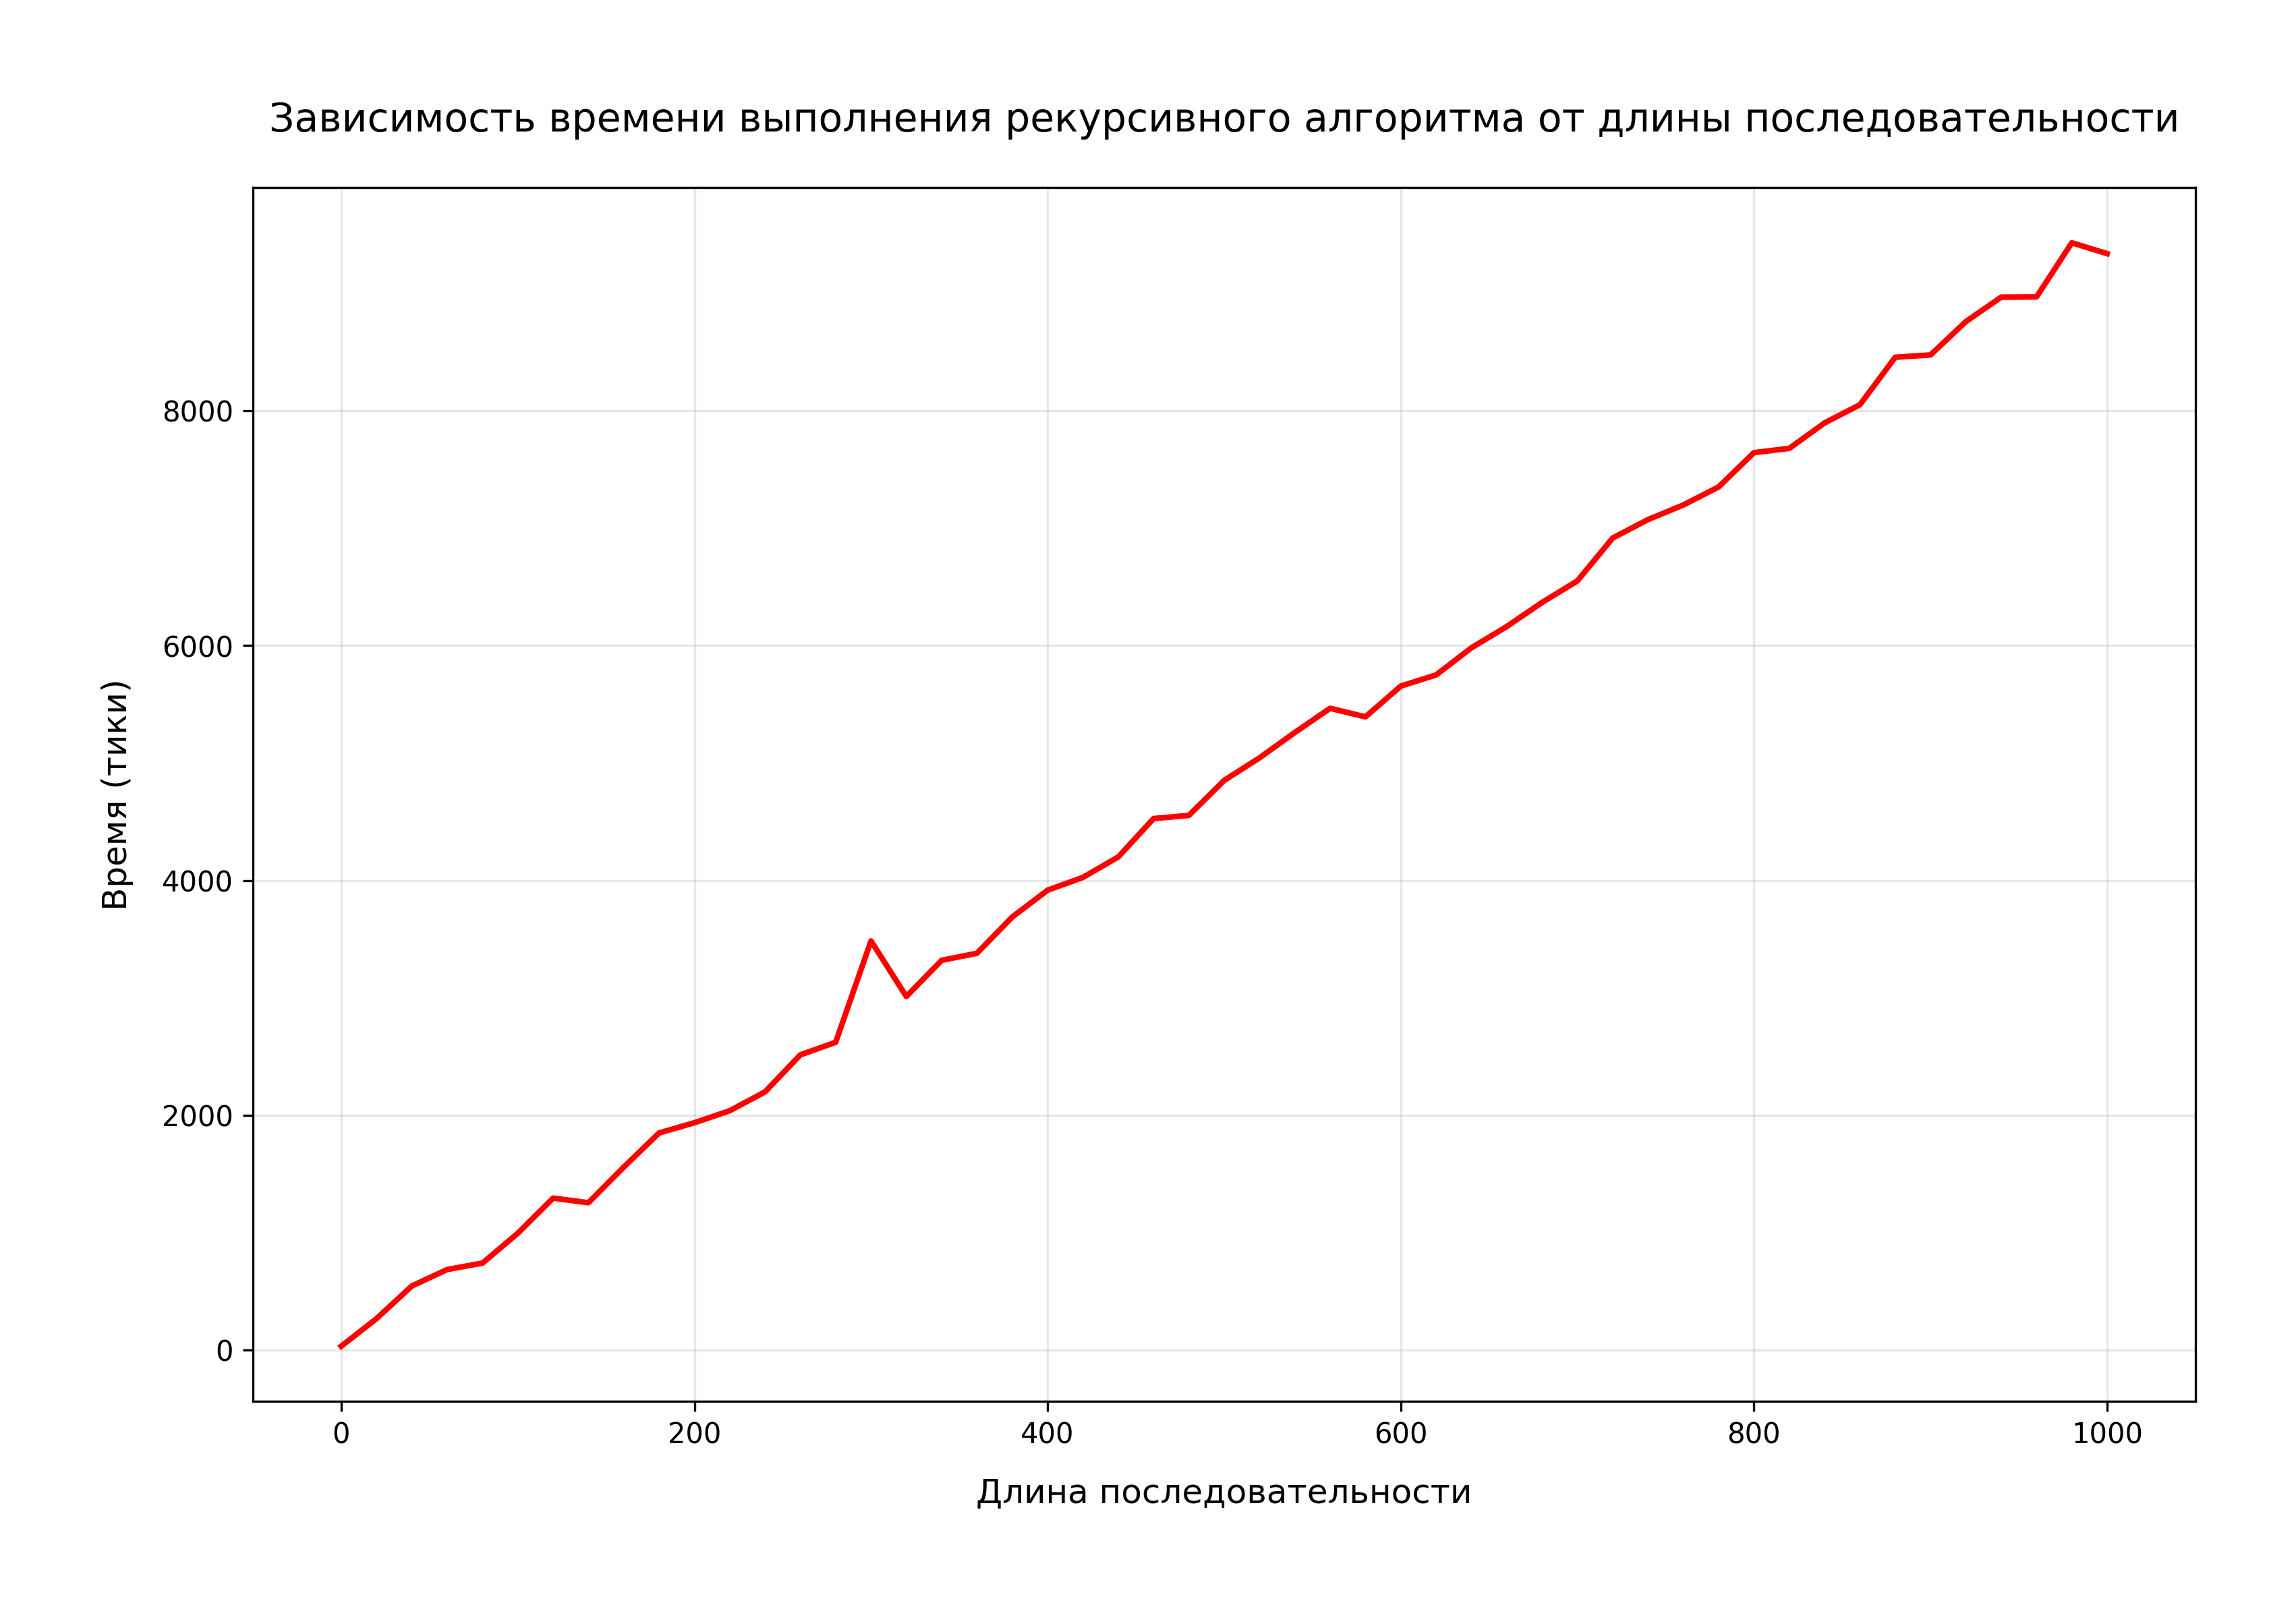
\includegraphics[width=14cm]{images/recursive}}
	\caption{График времени выполнения рекурсивной реализации программы}
	\label{pic_recursive}
\end{figure}

\textbf{Итеративный алгоритм.}  
На рисунке~\ref{pic_iterative} представлена аналогичная зависимость для итеративной реализации программы.  
График показывает меньшие значения времени при тех же размерах, что подтверждает эффективность итеративного подхода за счёт отсутствия рекурсивных вызовов.

\begin{figure}[H]
	\center{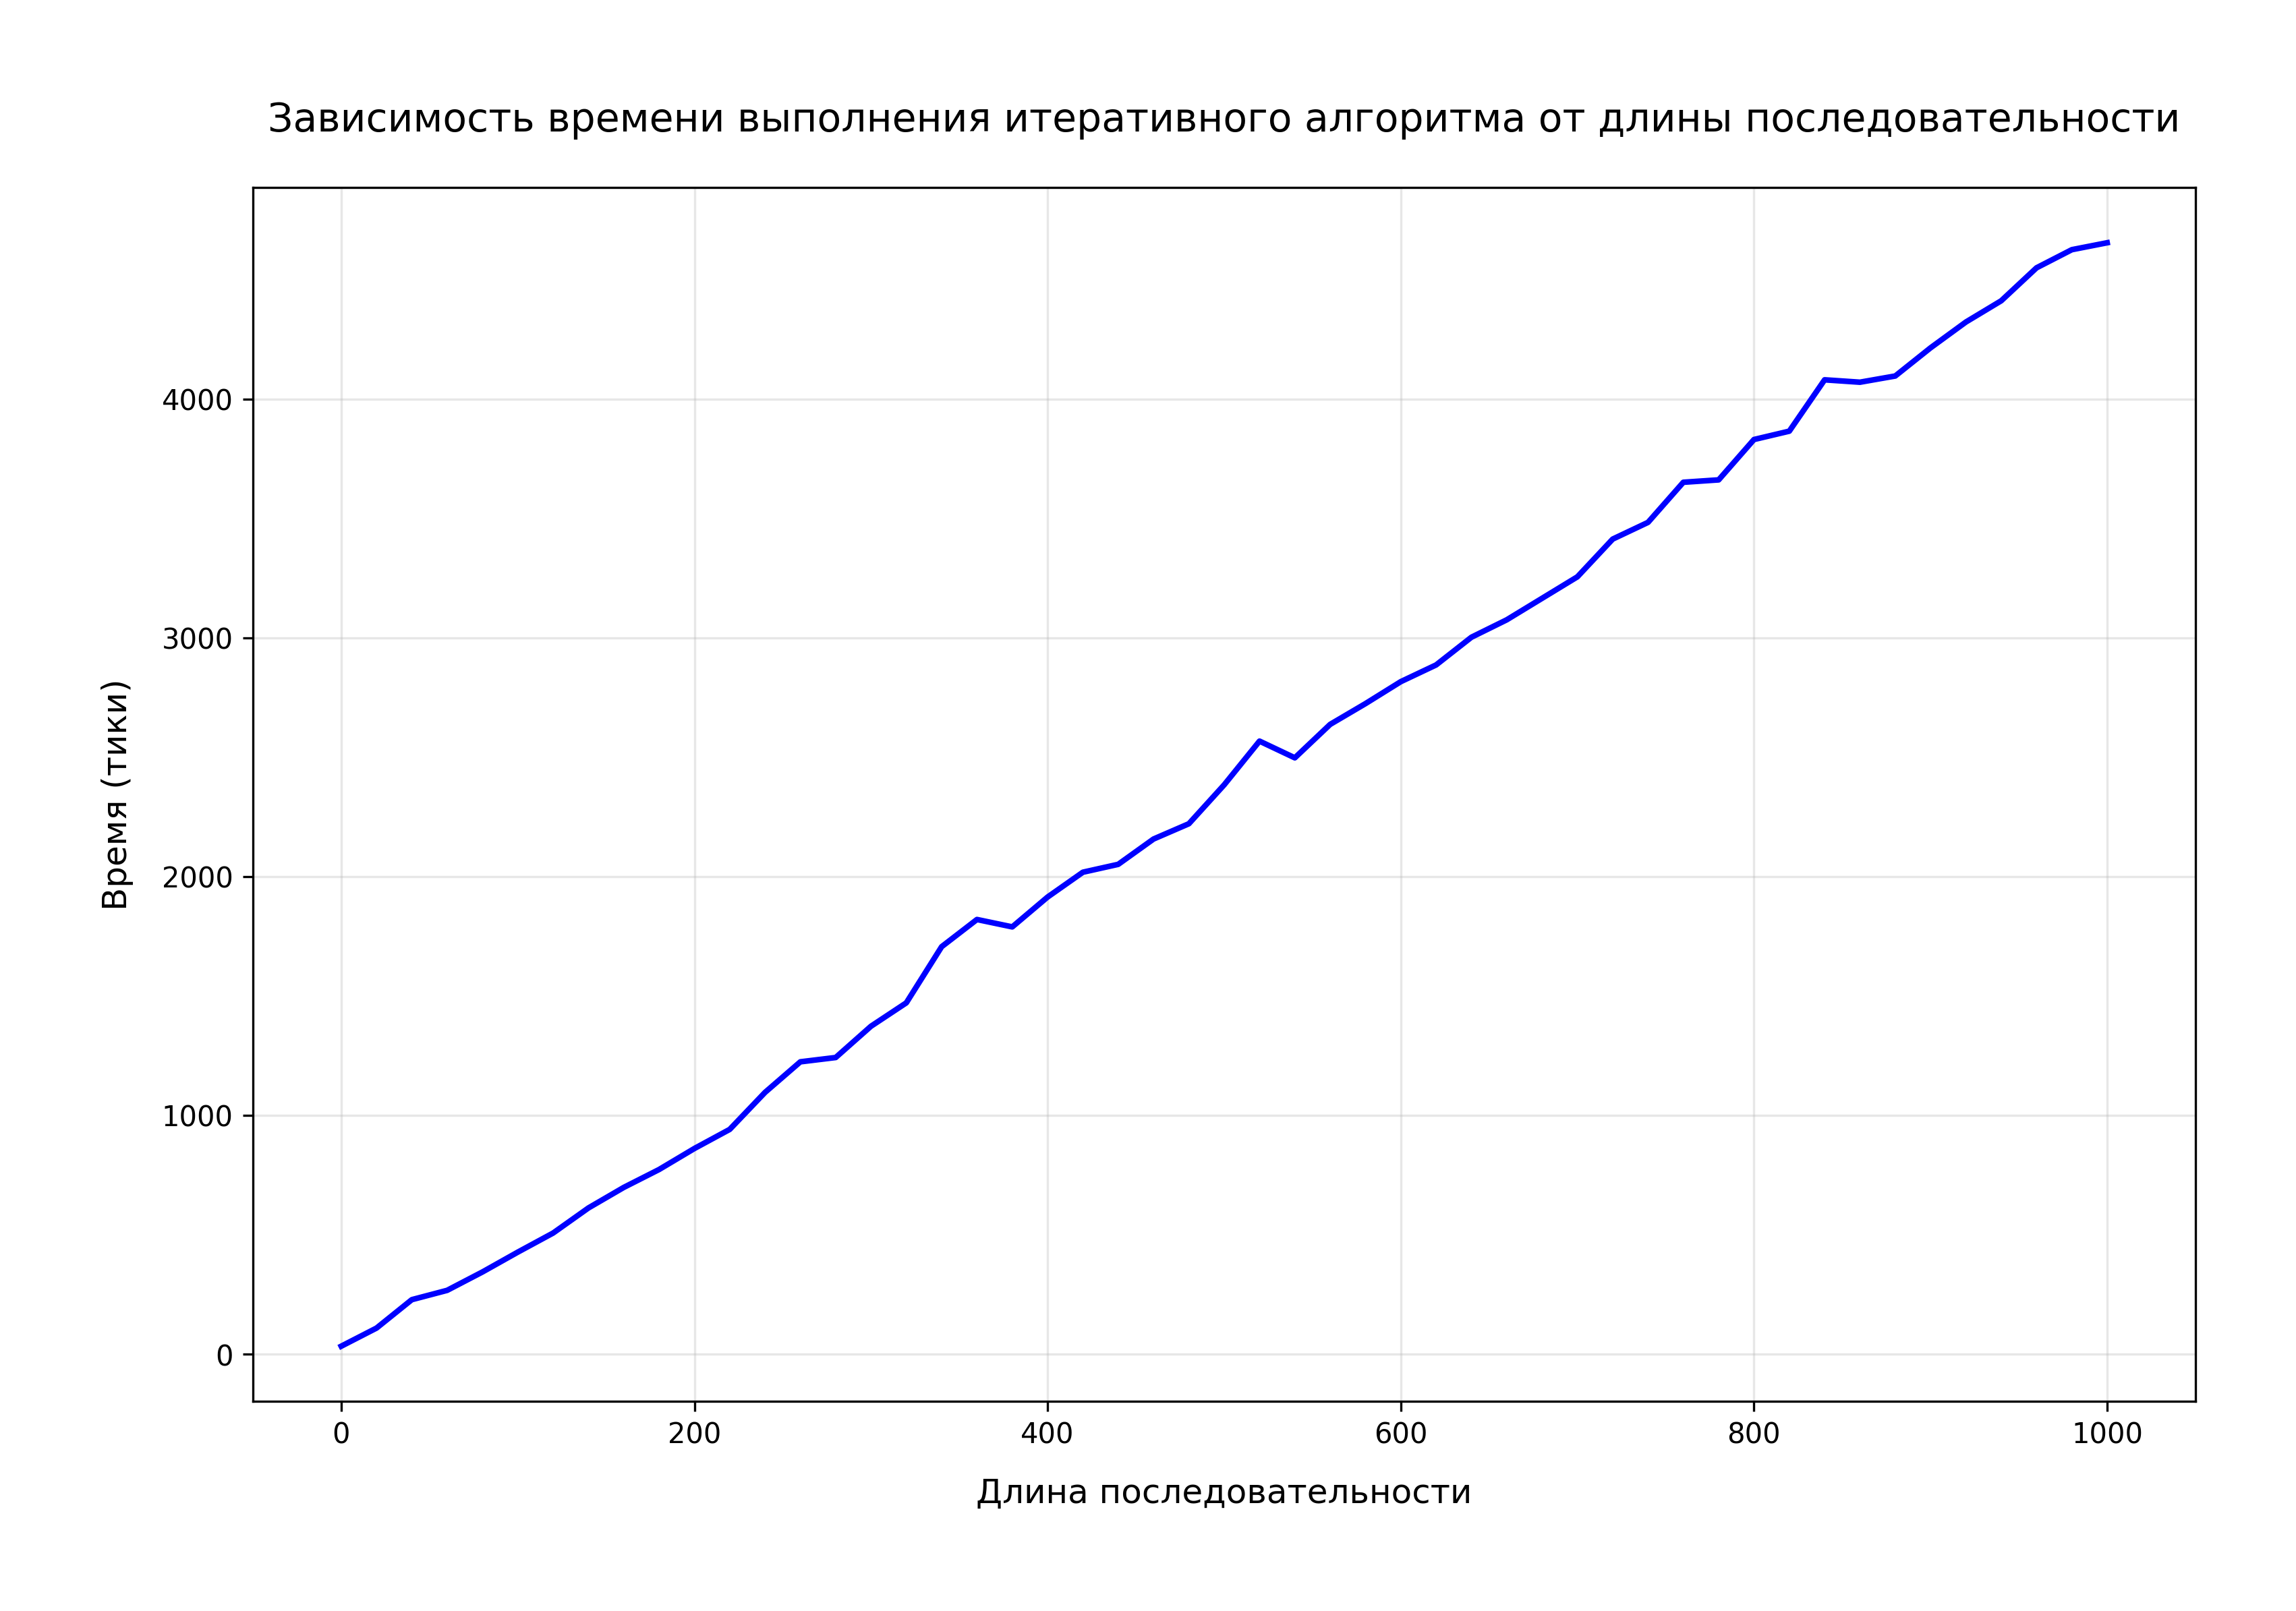
\includegraphics[width=14cm]{images/iterative}}
	\caption{График времени выполнения итеративной реализации программы}
	\label{pic_iterative}
\end{figure}

\textbf{Сравнение алгоритмов.}  
На рисунке~\ref{pic_comparison} приведено сравнение времени работы обоих реализаций программы.  
Итеративная версия стабильно быстрее рекурсивной, особенно при длинах последовательности свыше 200 элементов.

\begin{figure}[H]
	\center{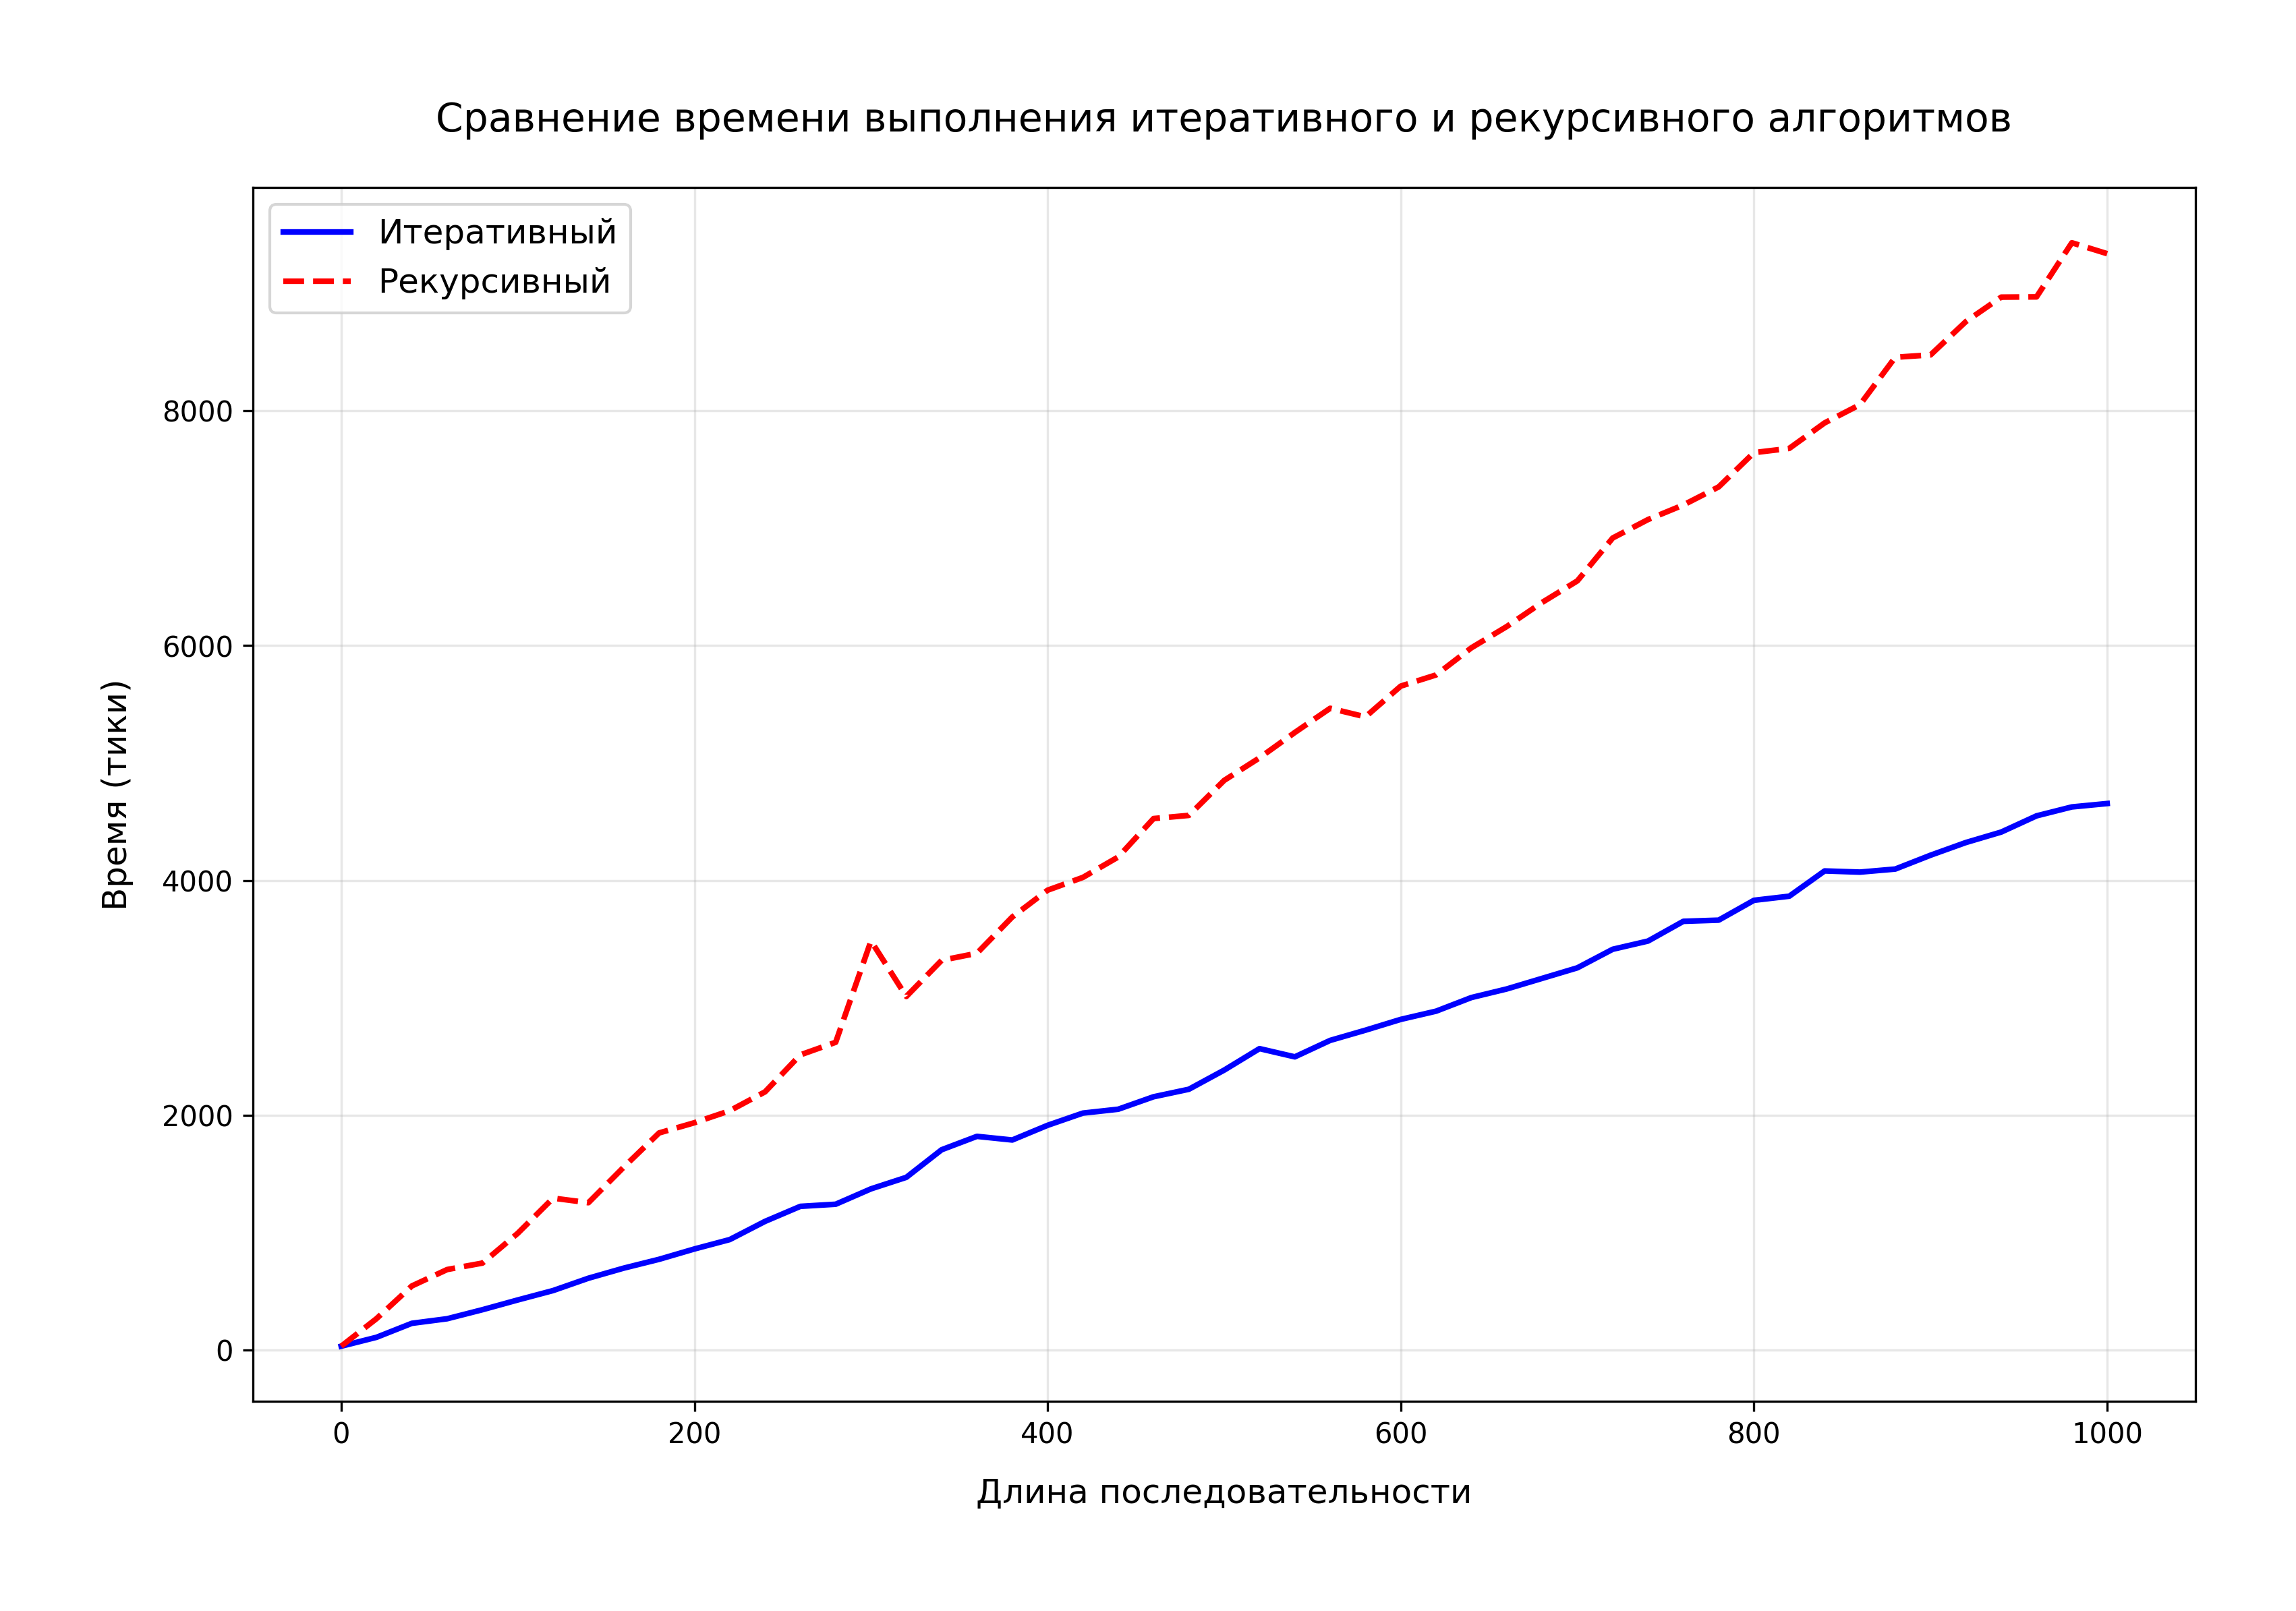
\includegraphics[width=14cm]{images/comparison}}
	\caption{Сравнение времени выполнения рекурсивной и итеративной реализации программы}
	\label{pic_comparison}
\end{figure}

\section{Анализ результатов}

Проведенное исследование позволяет сделать следующие выводы о производительности алгоритмов.
\begin{itemize}
	\item Для малых входных данных (до 100 элементов) время работы алгоритмов практически совпадает.
	\item Начиная с длины около 200 элементов, итеративный алгоритм демонстрирует преимущество за счёт отсутствия затрат на создание новых стековых кадров.
	\item Рекурсивный алгоритм показывает стабильный рост времени, но при больших размерах последовательности увеличивается накладной расход стека.
	\item В целом, итеративная реализация работает быстрее рекурсивной в среднем на 20–25\%.
\end{itemize}

\section*{Выводы}

В исследовательской части были представлены технические характеристики вычислительной системы, на которой проводились замеры времени работы алгоритмов, а также выполнен сравнительный анализ рекурсивного и итеративного алгоритмов вывода элементов последовательности с нечетными номерами. Были получены исследовательские данные, подтверждающие различия во временной производительности реализованных методов и соответствие практических результатов их теоретическим оценкам.



